\documentclass[tikz]{standalone}
\usepackage{bm}
\usetikzlibrary{patterns}
\begin{document}
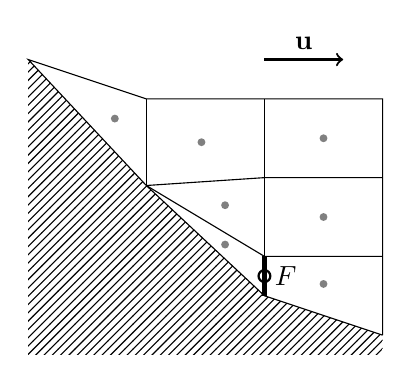
\begin{tikzpicture}[
  scale=0.5,
  cpnt/.style={fill=gray},
]

\draw [thick, ->] (6,7) -- (8,7) node [midway, anchor=south] {$\mathbf{u}$};

\draw (9,0) -- (9,6) -- (3,6) -- (0,7) -- (3,3.8) -- (6,1) -- (9,0);
\draw (3,6) -- (3,3.8);
\draw (6,6) -- (6,1);
\draw (9,2) -- (6,2) -- (3,3.8);
\draw (9,4) -- (6,4) -- (3,3.8);

\fill [pattern=north east lines] (0,7) -- (3,3.8) -- (6,1) -- (9,0) -- (9,-0.5) -- (0,-0.5) -- (0,7);

\draw [ultra thick] (6,1) -- (6,2);
\draw [thick] (6,1.5) circle [radius=0.15] node [anchor=west] {$F$};

\path [cpnt] (2.2,5.5) circle [radius=0.1];

\path [cpnt] (5,2.3) circle [radius=0.1];
\path [cpnt] (5,3.3) circle [radius=0.1];
\path [cpnt] (4.4,4.9) circle [radius=0.1];

\path [cpnt] (7.5,1.3) circle [radius=0.1];
\path [cpnt] (7.5,3) circle [radius=0.1];
\path [cpnt] (7.5,5) circle [radius=0.1];

\end{tikzpicture}
\end{document}
